\documentclass[class=minimal,border=0pt]{standalone}

\usepackage{tudfonts}

\usepackage{tikz}
\usetikzlibrary{calc}
\usetikzlibrary{matrix}
\usetikzlibrary{positioning}

\begin{document}

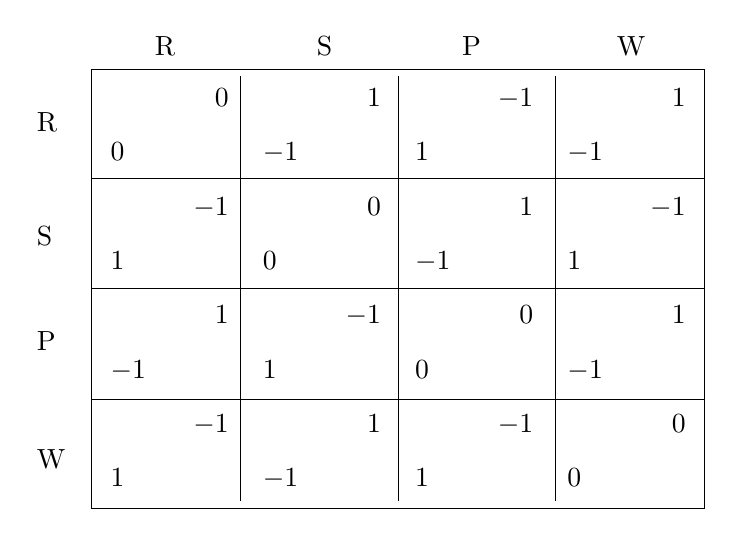
\begin{tikzpicture}

\matrix[matrix of math nodes,every odd row/.style={align=right},every even row/.style={align=left},every node/.style={text width=1.5cm},row sep=0.2cm,column sep=0.2cm] (m) {
$0$&$1$&$-1$&$1$\\
$0$&$-1$&$1$&$-1$\\
$-1$&$0$&$1$&$-1$\\
$1$&$0$&$-1$&$1$\\
$1$&$-1$&$0$&$1$\\
$-1$&$1$&$0$&$-1$\\
$-1$&$1$&$-1$&$0$\\
$1$&$-1$&$1$&$0$\\
};
\draw (m.north east) rectangle (m.south west);
\draw (m.north west)--(m.north west);
\draw (2,2.7) -- (2,-2.7);
\draw (0,2.7) -- (0,-2.7);
\draw (-2,2.7) -- (-2,-2.7);

\draw (3.9,1.4) -- (-3.9,1.4);
\draw (3.9,0) -- (-3.9,0);
\draw (3.9,-1.4) -- (-3.9,-1.4);


\coordinate (a) at ($(m.north west)!0.12!(m.north east)$);
\coordinate (b) at ($(m.north west)!0.38!(m.north east)$);
\coordinate (c) at ($(m.north west)!0.62!(m.north east)$);
\coordinate (d) at ($(m.north west)!0.88!(m.north east)$);
\node[above=5pt of a,anchor=base] {R};
\node[above=5pt of b,anchor=base] {S};
\node[above=5pt of c,anchor=base] {P};
\node[above=5pt of d,anchor=base] {W};

\coordinate (e) at ($(m.north west)!0.12!(m.south west)$);
\coordinate (f) at ($(m.north west)!0.38!(m.south west)$);
\coordinate (g) at ($(m.north west)!0.62!(m.south west)$);
\coordinate (h) at ($(m.north west)!0.888!(m.south west)$);
\node[left=2pt of e,text width=.5cm]  {R};
\node[left=2pt of f,text width=.5cm]  {S};
\node[left=2pt of g,text width=.5cm]  {P};
\node[left=2pt of h,text width=.5cm]  {W};


\end{tikzpicture}

\end{document}
